\documentclass[a4paper, 12pt]{article}
\usepackage{physics, amsmath, amsfonts, fixmath, geometry, tikz, pgf, multirow, hyperref, amsfonts,amssymb, mathtools, physics, xcolor, siunitx, subcaption,tcolorbox}


\usepackage{graphicx}
\usepackage{braket}
\usepackage{enumitem,hyperref,dsfont}
\usepackage[linewidth= 2pt]{mdframed}
\usepackage{colortbl}
\usepackage{xepersian}
\setdigitfont{XB Niloofar}
\settextfont[]{XB Niloofar}
\deflatinfont\enfont[Scale=1]{Times New Roman}
\newcommand{\pcur}[0]{\lr{Page curve}}
\newcommand{\mycomment}[1]{}
\title{\textbf{
  آیا گروه خارج قسمتی با زیرگروهی از گروه اولیه یکریخت است؟
}}
\author{حسین محمدی
\\}
\newtcolorbox{boxes}[3][]
{
	colframe = #2!25,
	colback  = #2!10,
	coltitle = #2!40!black,  
	title    = {\textbf{#3}},
	#1,
}

\begin{document}
\maketitle

\begin{mdframed}
	برخی از شما نکته‌ای را به من تذکر دادید که به اشتباه در کلاس درس گفته شد. این‌جا سعی می‌کنیم آن را تصحیح کنیم.
\end{mdframed}

آیا برای زیرگروه بهنجار
$H \trianglelefteq G$، گروه خارج قسمتی
$\frac{G}{H}$
با زیرگروهی از خود 
$G$ یکریخت است؟

\textbf{نه لزوما.}
 مثلا گروه $Q$ یا کواترنیون‌ها را در نظر بگیرید و زیرگروه 
 $H=\{1,-1\}$
 از آن که یک زیرگروه بهنجار است. می‌دانیم که گروه خارج‌قسمتی $\frac{G}{H}$ از همدسته‌های این زیرگروه تشکیل شده است؛ پس داریم:
 \[
 \frac{Q}{H} = \{
 \{1,-1\} , \{i,-i\} , \{j,-j\},\{k,-k\}
 \}
 \]

جدول ضرب آن در پایین آمده
است.
\begin{figure}
	\centering
	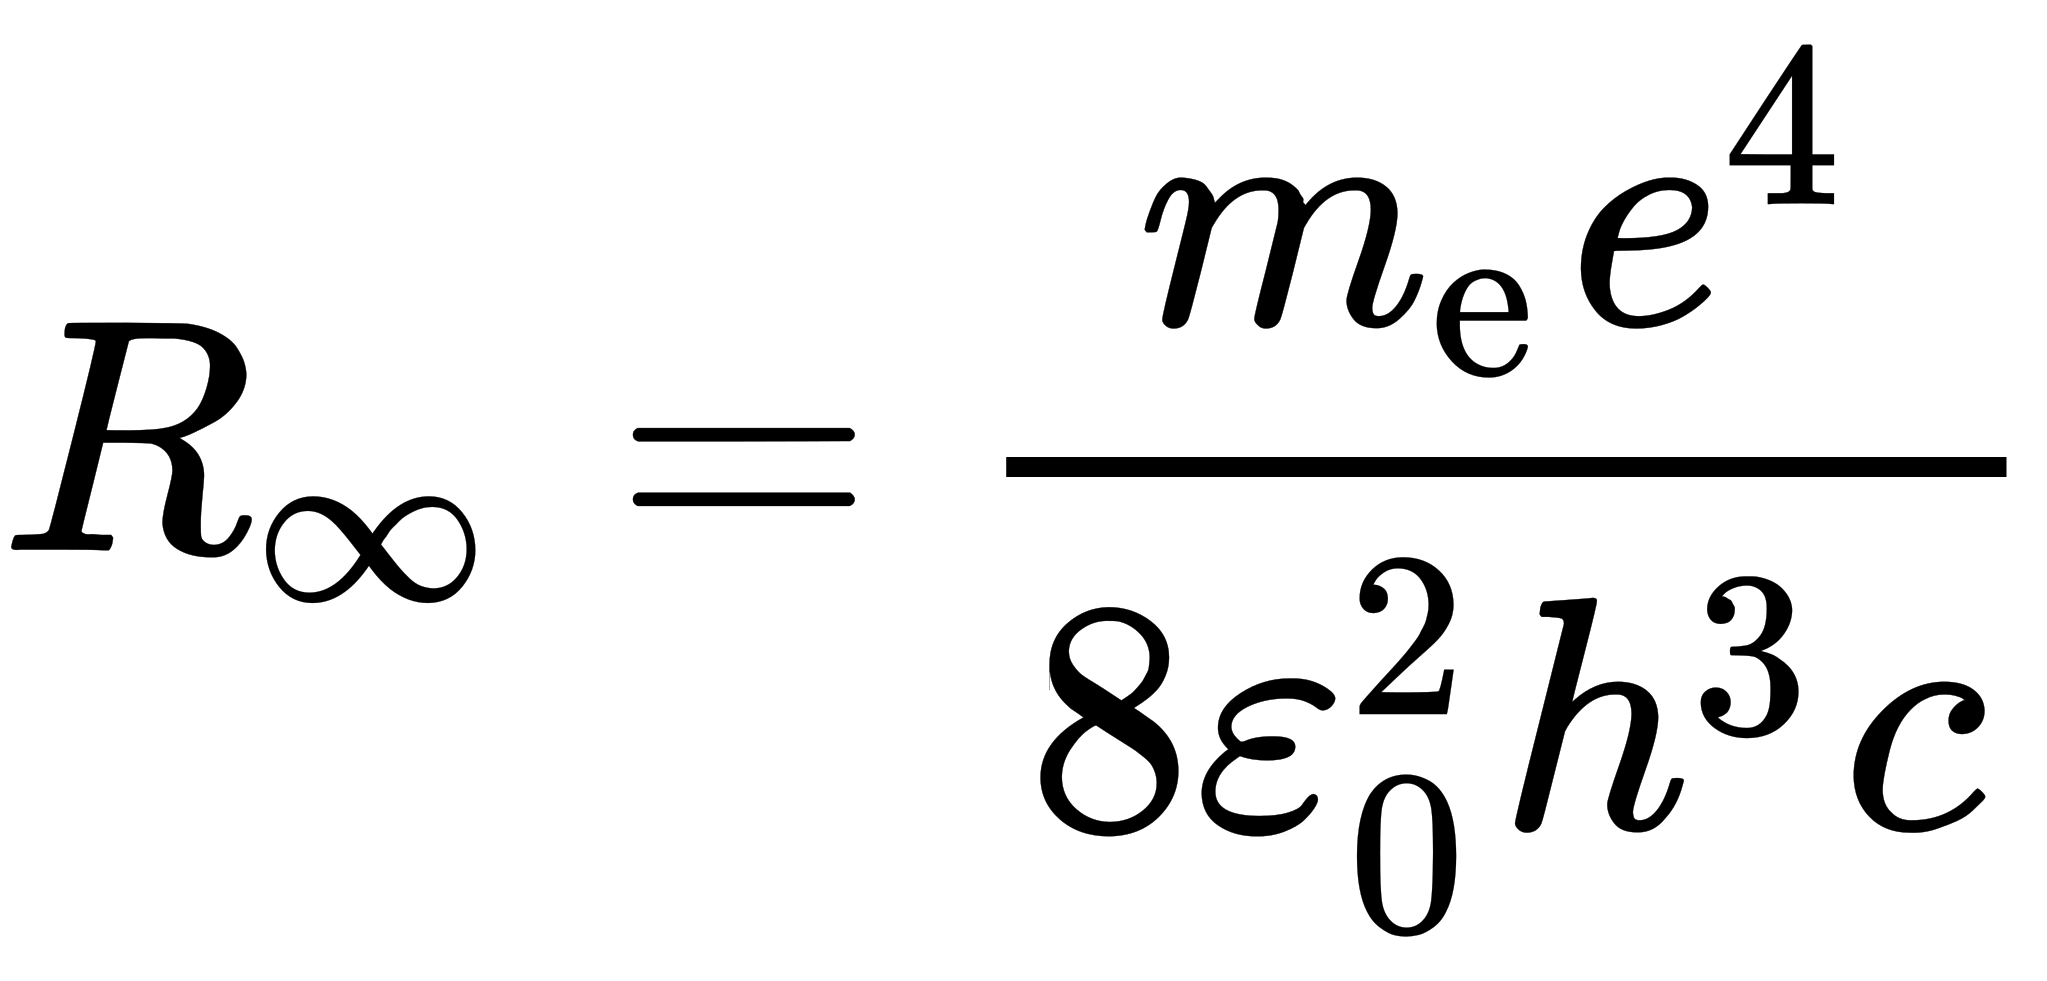
\includegraphics[width=22em]{1.png}
	\caption*{جدول ضرب گروه خارج قسمتی}
	\label{b}
\end{figure}


همانطور که می‌بینید این گروه چهار عضوی، هیچ عضو مرتبه‌چهاری ندارد و یکریخت با گروه کلاین، یعنی 
$\mathbb{Z}_2 \times \mathbb{Z}_2$
است.

این در حالی است که تمام زیرگروه‌های چهارعضوی گروه کواترنیون به شکل زیر است:
\begin{equation*}
	\begin{aligned}
		K_1 &= \{1,-1,i,-i\} = \left< i\right> \\
			K_2 &= \{1,-1,j,-j\} = \left< j\right> \\
				K_3 &= \{1,-1,k,-k\} = \left< k\right> \\
	\end{aligned}
\end{equation*}
یعنی همگی دوری از مرتبه چهار هستند. پس لزوما زیرگروه $K$ وجود ندارد که 
$\frac{G}{H} \simeq K$.

\vspace{3em}
\noindent
یا حتی مثالی ساده‌تر هم وجود دارد. گروه $G = \mathbb{Z} $ با عمل جمع و زیر گروه 
 $H = 2\mathbb{Z} \trianglelefteq G$
 متشکل از اعداد زوج را در نظر بگیرید. می‌دانیم که 
 \[
 \frac{G}{H} = \frac{\mathbb{Z}}{2\mathbb{Z}} \simeq \mathbb{Z}_2
 \]
 اما هیچ زیرگروه دو‌عضوی‌ای از گروه $\mathbb{Z}$ نداریم؛ چون هیچ عضوی با مرتبه‌ی دو در این گروه نیست.
 
 
 \begin{boxes}{black}{تبصره}
 	به سادگی می‌توانید نشان دهید وقتی که گروه $G$ آبلی و متناهی باشد؛ هر زیرگروه خارج قسمتی از آن همریخت با یک زیرگروه از گروه اولیه است.
 \end{boxes}
\end{document}